\documentclass[10pt,a4paper]{article}
\usepackage[utf8]{inputenc}
\usepackage{amsmath}
\usepackage{amsfonts}
\usepackage{booktabs}
\usepackage[margin=1in]{geometry}
\usepackage{amssymb}
\usepackage{tikz}
\author{Joel Mizzoni (jmizzoni), Patrick White (ps2white)}
\begin{document}
\title{ECE358 S'16 Assignment 4}
\maketitle
\section{}
\subsection*{a}
\begin{itemize}
    \item[A] 1.2.3.0/30
    \item[B] 1.2.3.0
    \item[C] 1.2.3.1
    \item[D] 1.2.3.2
    \item[E] 1.2.3.4/30
    \item[F] 1.2.3.4
    \item[G] 1.2.3.5
    \item[H] 1.2.3.6
    \item[I] 10.10.0.0/16
    \item[J] 10.20.0.0/16
    \item[K] 1.2.3.8/30
    \item[L] 1.2.3.8
    \item[M] 1.2.3.9
    \item[N] 1.2.3.10
    \item[O] 10.30.0.0/16
    \item[P] 10.40.0.0/16
\end{itemize}
\subsection*{b}
\subsubsection*{i: Sales Router}
\begin{tabular}{c c c}
    \toprule
    \textbf{Prefix} & \textbf{Next Hop} & \textbf{Interface} \\\midrule
    1.2.3.0/30 & myself & C \\
    1.2.3.4/30 & myself & F \\
    1.2.3.8/30 & 1.2.3.2 & C \\
    0.0.0.0/0 & 1.2.3.0 & C \\\bottomrule
\end{tabular}
\subsubsection*{ii: Marketing Router}
\begin{tabular}{c c c}
    \toprule
    \textbf{Prefix} & \textbf{Next Hop} & \textbf{Interface} \\\midrule
    1.2.3.0/30 & myself & D \\
    1.2.3.4/30 & 1.2.3.1 & D \\
    1.2.3.8/30 & myself & L \\
    0.0.0.0/0 & 1.2.3.0 & D \\\bottomrule
\end{tabular}
\section{}
\begin{tabular}{c c c c}
    \toprule
    \textbf{Identification} & \textbf{More Fragments} & \textbf{Fragment Offset} & \textbf{Total Length} \\\midrule
    abcd & 1 & 0 & 500 \\
    abcd & 1 & 60 & 500 \\
    abcd & 1 & 120 & 36 \\
    abcd & 0 & 122 & 844 \\\bottomrule
\end{tabular}
\section{}
\begin{itemize}
    \item[a.] The value of the checksum received by $D$ is not necessarily the same as the checksum sent by $S$. This is because the checksum is recalculated at each hop, and at each hop the header changes (at minimum, the TTL field changes). It is possible for the value to be the same (multiple values of the header map to the same value for the checksum) but unless the source and destination are on the same physical network (and there are no hops between them) it is unlikely the header value remains unchanged.
    \item[b.] Alice is incorrect. Consider the initial header bytes \texttt{0x0000 5555 5555 5555 5555}. The sum of each 16-bit pair is \texttt{0x15554}. Adding the carry back gives \texttt{0x5555}. Taking the 1s complement gives \texttt{0xaaaa}, the checksum value sent by the source.
        Not consider that three of the bytes become flipped in transit, so the header becomes \texttt{0x0000 5554 5557 5554 5555}. The sum of each 16-bit pair is \texttt{0x15554}. Adding the carry back gives \texttt{0x5555}. Taking the 1s complement gives \texttt{0xaaaa}, the checksum value sent by the source, even though an odd number of bits were flipped.
    \item[c.] The value of the checksum received by $D$ is not necessarily the same as the checksum sent by $S$. This is because a NAT server can rewrite the UDP header of a packet, which includes recomputing the checksum. Although the UDP header is not recomputed at every hop, it can be recomputed whenever it passes through a NAT.
    \item[d.] It is not necessarily true that if a response is not received, the MTU is not supported. It is possible that the echo service is not working or not enabled on the remote host, so even though it receives the (non-fragmented) packet destined for port 7, it does not reply.
\end{itemize}
\section{}
If $u\rightsquigarrow x \rightarrow y$ is a shortest path, then the length of this path is $\delta(y)$. If before $x$ entered $N'$, $D(y)$ was some value greater than $\delta(y)$, then after $x$ is added to $N'$ the value of $D(y)$ will be updated to $\delta(y)$. Therefore at this stage in the algorithm, $D(y) = \delta(y)$.
\section{}
First, we assert that any path (and therefore the shortest path) from $x$ to $y$ includes exactly one of the edges from $x$ to a vertex in $neigh(x)$.
Secondly, the shortest path from $x$ to $y$ including neighbor $v$ of $x$ is $x \rightarrow v \rightsquigarrow y$ where $v \rightsquigarrow y$ is the shortest path from $v$ to $y$. This path has length $c(x,v) + d_v(y)$.
From the previous two, the shortest path from $x$ to $y$ is $x \rightarrow v \rightsquigarrow y$ where $v\in neigh(x)$.
Therefore, the length of the shortest path from $x$ to $y$ is $\min\limits_{v\in neigh(x)}\left\{c(x,v) + d_v(y)\right\}$.
\section{}
When using the distance vector algorithm from an initial state where all path lengths are unknown, after $N$ iterations, each node will be aware of the shortest path to each node consisting of $N$ edges. This means the number of iterations it will take to converge is equal to the longest (in # of edges) shortest path in the network plus 1 (since one more iteration has to occur in order for the last nodes to update to broadcast one last message). The greatest number of edges a shortest path can have is $N - 1$, we will converge in at most $N$ iterations.
\section{}
A network that would cause this to occur looks like this:

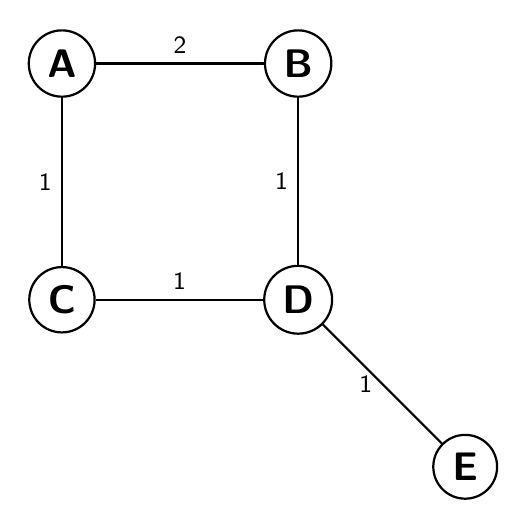
\begin{tikzpicture} [auto, node distance=3cm, every loop/.style={},
                    thick,main node/.style={circle,draw,font=\sffamily\Large\bfseries}]
    \node[main node] (1){A};
    \node[main node] (2)[right of=1]{B};
    \node[main node] (3)[below of=1]{C};
    \node[main node] (4)[below of=2]{D};
    \node[main node] (5)[below right of=4]{E};

    \path[every node/.style={font=\sffamily\small}]
    (1) edge node [above] {2} (2)
        edge node [left] {1} (3)
    (2) edge node [left] {1} (4)
    (3) edge node [above] {1} (4)
    (4) edge node [left] {1} (5);
\end{tikzpicture}
If the cost from $D \leftrightarrow E$ is updated to some large value (e.g. 50), assume that D notices the change first.
The first update will result in D routing through C to get to E (assuming a path cost of 3). D then broadcasts the update to B and C.
Assume C receives the update first. Using poisoned reverse, C will choose to route to E through A (cost 4). 
A will then choose to route through B (cost 4), and then B will still think it can route through D with a cost of 2.
At this point, before the other updates are processed, the loop has started, and a packet will travel from $A \rightarrow C \rightarrow D \rightarrow B \rightarrow A \ldots$ until the routing tables converge to taking the path from D to E.

\end{document}
